\documentclass[handout,nooutcomes]{ximera}
%% handout
%% space
%% newpage
%% numbers
%% nooutcomes

%I added the commands here so that I would't have to keep looking them up
%\newcommand{\RR}{\mathbb R}
%\renewcommand{\d}{\,d}
%\newcommand{\dd}[2][]{\frac{d #1}{d #2}}
%\renewcommand{\l}{\ell}
%\newcommand{\ddx}{\frac{d}{dx}}
%\everymath{\displaystyle}
%\newcommand{\dfn}{\textbf}
%\newcommand{\eval}[1]{\bigg[ #1 \bigg]}

%\begin{image}
%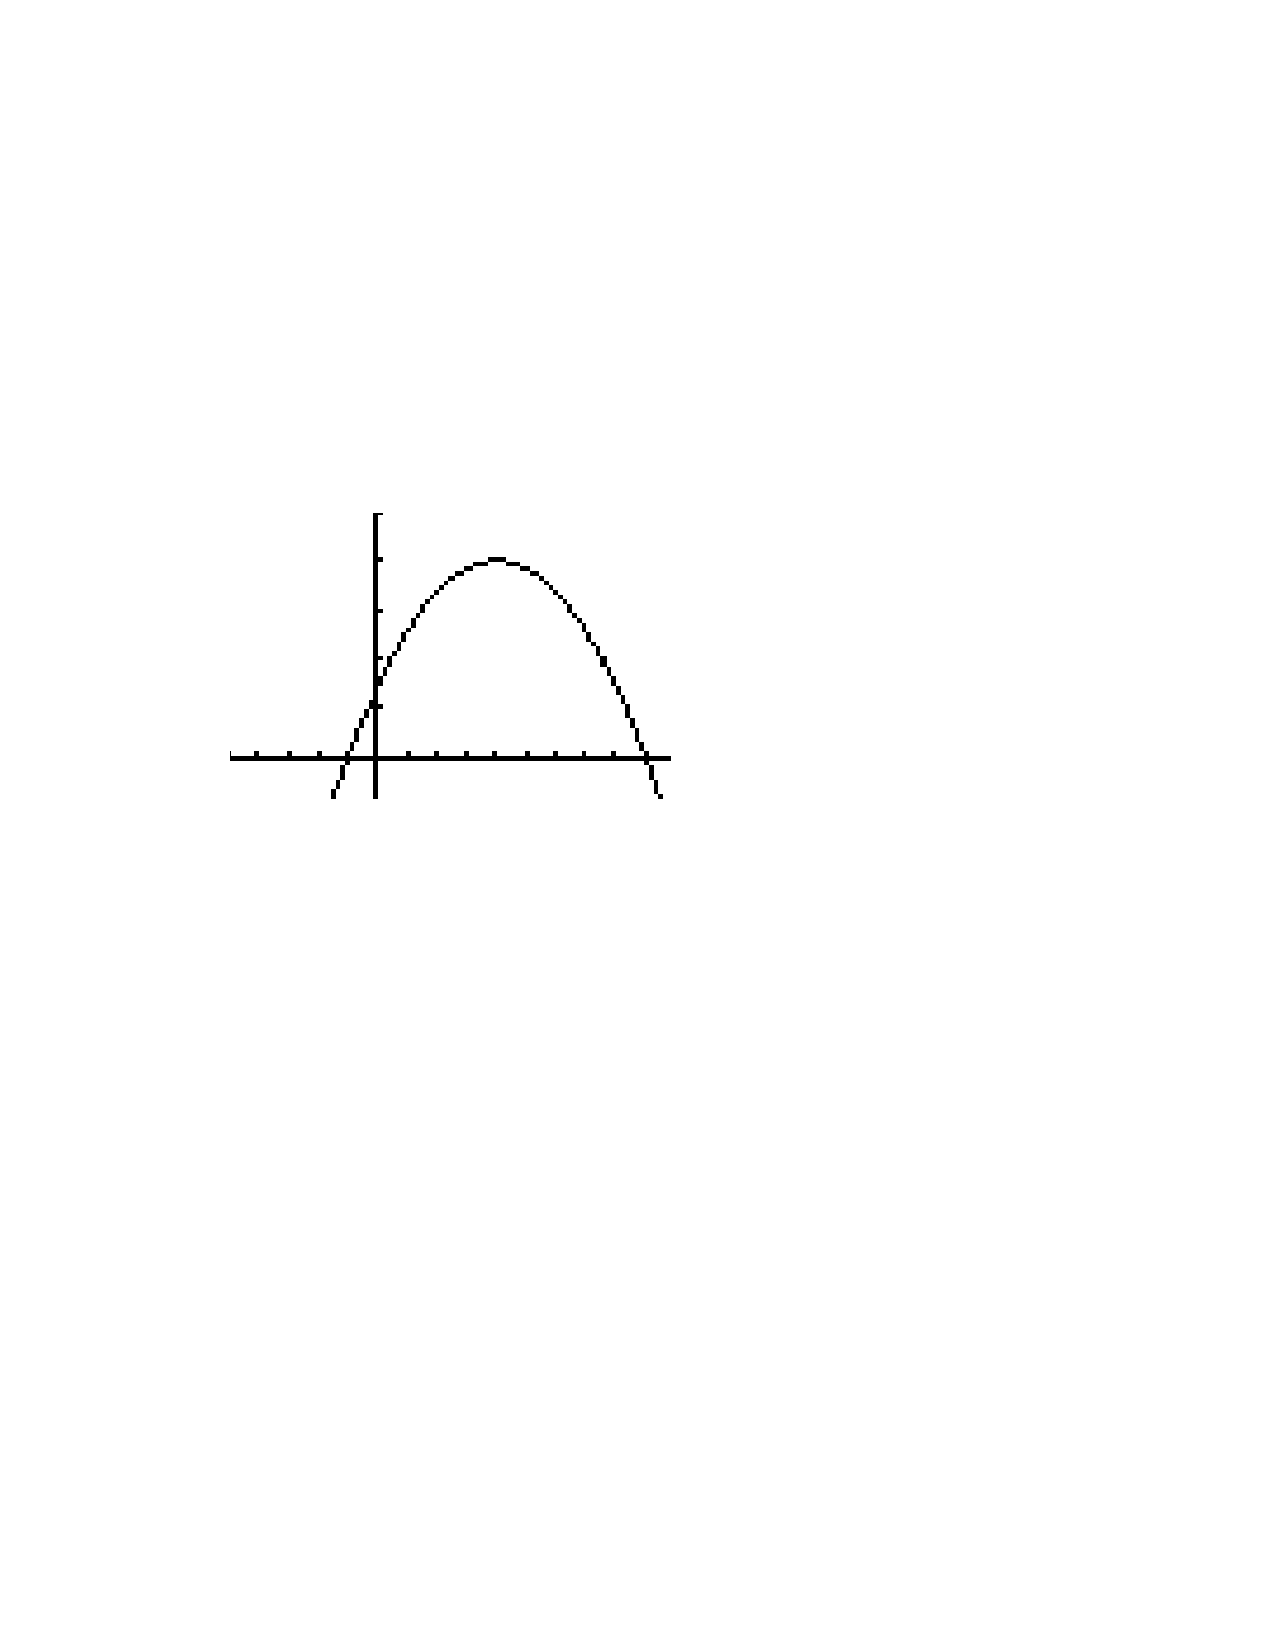
\includegraphics[trim= 170 420 250 180]{Figure1.pdf}
%\end{image}


\newcommand{\RR}{\mathbb R}
\renewcommand{\d}{\,d}
\newcommand{\dd}[2][]{\frac{d #1}{d #2}}
\renewcommand{\l}{\ell}
\newcommand{\ddx}{\frac{d}{dx}}
\newcommand{\dfn}{\textbf}
\newcommand{\eval}[1]{\bigg[ #1 \bigg]}

\usepackage{multicol}

\renewenvironment{freeResponse}{
\ifhandout\setbox0\vbox\bgroup\else
\begin{trivlist}\item[\hskip \labelsep\bfseries Solution:\hspace{2ex}]
\fi}
{\ifhandout\egroup\else
\end{trivlist}
\fi} %% we can turn off input when making a master document

\title{Recitation \#19 - 4.5 Linear Approximations and Differentials}  

\begin{document}
\begin{abstract}		\end{abstract}
\maketitle

\section*{Warm up:} 
By using linear approximation, determine which of the following is the best estimate of $e^{0.002}$.
	\begin{enumerate}
	\item[(a)]  1.00100050016679834166
	\item[(b)]  1.00200200133400026675
	\item[(c)]  1.00300450450337702601
	\item[(d)]  1.02020134002675581016
	\end{enumerate}
	
		\begin{freeResponse}
		Let $f(x) = e^x$ and $a=0$.  Then since $f'(x) = e^x$, we have that
		\begin{align*}
		L(x) &= f(a) + f'(a)(x-a) \\
		&=  f(0) + f'(0)(x-0) \\
		&= e^0 + e^0x \\
		&= 1 + x
		\end{align*}
		Then since $L(0.002) = 1 + 0.002 = 1.002$, the answer is (b).
		\end{freeResponse}	
		
		
		

	
	
	
	
	

\section*{Group work:}



%problem 1
\begin{problem}
Complete steps (i)-(vii) below in order to estimate the following values using linear approximation:
$$ (a) \; \cos \left( \frac{31 \pi}{180} \right)	\hskip 100pt	(b) \; \sqrt[3]{8.13} $$
	\begin{enumerate}
	\item[i.]  Identify the function, $f(x)$.
	\item[ii.]  Find the nearby value where the function can be easily calculated, $x=a$.
	\item[iii.]  Find $\Delta x=dx$.
	\item[iv.]  Find the linear approximation equation, $L(x)$.  
	\item[v.]  Compute the approximate value of the expression using the linear approximation.
	\item[vi.]  Compare the approximated value to the value given by your calculator.
	\item[vii.]  Compare $dy$ and $\Delta y$ using the value given by your calculator.
	\end{enumerate}
		\begin{freeResponse}
		(a)  $ \cos \left( \frac{31 \pi}{180} \right)$
			\begin{enumerate}
			\item[i.]  $f(x) = \cos x$
			\item[ii.]  $a = \frac{30 \pi}{180} = \frac{\pi}{6}$
			\item[iii.]  $\Delta x = \frac{31 \pi}{180} - \frac{\pi}{6} = \frac{\pi}{180}$
			\item[iv.]  
				\begin{align*}
				L(x) &= f\left( \frac{\pi}{6} \right) + f^\prime \left(\frac{\pi}{6} \right) \left( x - \frac{\pi}{6} \right) \\
				&=  \cos \left( \frac{\pi}{6} \right) - \sin \left(\frac{\pi}{6} \right) \left( x - \frac{\pi}{6} \right) \\
				&=  \frac{\sqrt{3}}{2} - \frac{1}{2} \left( x - \frac{\pi}{6} \right) 
				\end{align*}
			\item[v.]   
				\begin{align*}
				L \left( \frac{31 \pi}{180} \right) &= \frac{\sqrt{3}}{2} - \frac{1}{2} \left( \frac{31 \pi}{180} - \frac{\pi}{6} \right) \\
				&=  \frac{\sqrt{3}}{2} - \frac{1}{2} \left( \frac{\pi}{180} \right) \\
				&= \frac{1}{2} \left( \sqrt{3} - \frac{\pi}{180} \right) \\
				&\approx 0.857299
				\end{align*}
			\item[vi.]  $\cos \left( \frac{31 \pi}{180} \right) \approx 0.857167$
			\item[vii.]  
			$$ dy = L\left( \frac{31\pi}{180} \right) - L \left( \frac{\pi}{6} \right) \approx -0.008727 $$
			$$ \Delta y = \cos \left( \frac{31 \pi}{180} \right) - \cos \left( \frac{\pi}{6} \right) \approx -0.008858 $$
			\end{enumerate}
			
		(b)  $ \sqrt[3]{8.13}$
			\begin{enumerate}
			\item[i.]  $f(x) = \sqrt[3]{x}$.
			\item[ii.]  $a=8$.
			\item[iii.]  $\Delta x = 8.13 - 8 = 0.13$.
			\item[iv.]  
				\begin{align*}
				L(x) &= f(8) + f^\prime (8) (x-8) \\
				&= \sqrt[3]{8} + \frac{1}{3 (\sqrt[3]{8})^2} \left( x - 8 \right) \\
				&= 2 + \frac{1}{12} (x-8) 
				\end{align*}
			\item[v.]  
				\begin{align*}
				L(8.13) &= 2 + \frac{1}{12} (8.13 - 8) \\
				&= 2 + \left( \frac{1}{12} \right) \left( \frac{13}{100} \right) \\
				&= 2 + \frac{13}{1200} = \frac{2413}{1200} \\
				&\approx 2.010833
				\end{align*}
			\item[vi.]  $\sqrt[3]{8.13} \approx 2.010775$.
			\item[vii.]  
			$$ dy = L(8.13) - L(8) \approx 0.010833 $$
			$$ \Delta y = \sqrt[3]{8.13} - \sqrt[3]{8} \approx 0.010775 $$
			\end{enumerate}
		\end{freeResponse}
		
		
\end{problem}







\newpage








%problem 2
\begin{problem}
Consider the graph of $f^\prime (x)$ given below.  Suppose that $f(2) = 4$.  Approximate 
$f(1.98)$ and $f(2.02)$ as best as you can.  Determine whether your approximations are over or under estimates.  
Suppose you also know $f(3) = 7$.  
Can you approximate $f(2.98)$ and $f(3.02)$?  
Explain your answer.

	\begin{image}
	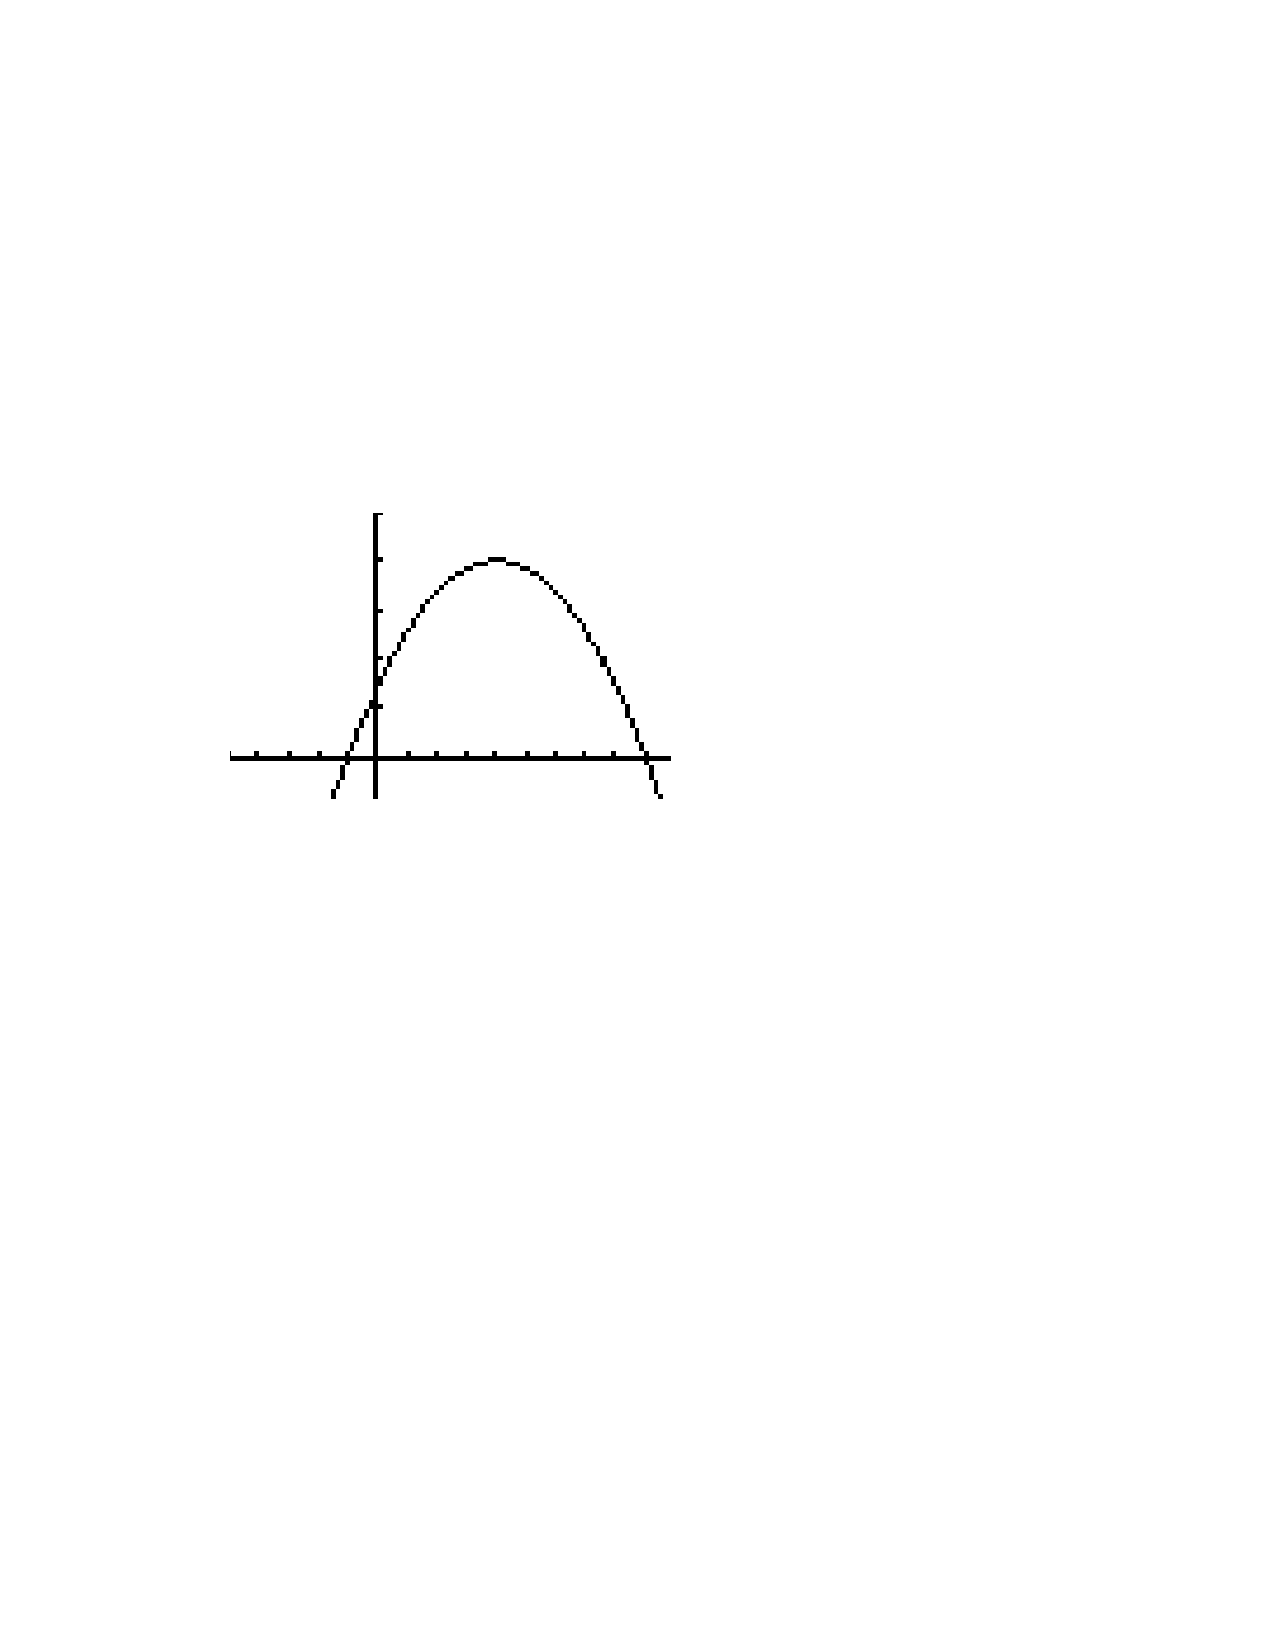
\includegraphics[trim= 60 420 250 200]{Figure1.pdf}
	\end{image}
	
		\begin{freeResponse}
		$f(2) = 4$ and $f^\prime (2)$ looks to be about $1.75 = \frac{7}{4}$.  So $L(x) = 4 + \frac{7}{4} (x-2)$.  Therefore
			\begin{align*}
			L(1.98) &= 4 + \frac{7}{4} (1.98-2) = 4 + \frac{7}{4} (-0.02) = 4-0.035 = 3.965 \\
			L(2.02) &= 4 + \frac{7}{4} (2.02-2) = 4 + \frac{7}{4} (0.02) = 4+0.035 = 4.035
			\end{align*}
		So $f(1.98)\approx 3.965$ and $f(2.02)\approx 4.035$ 
Since $f^\prime$ is decreasing, the graph of $f$ is concave down.  Therefore the graph of $L(x)$ lies above the graph of $f$ near $x=2$.  This means that these are overestimates.

		$f(3)=7$ and $f^\prime (3)=0$ 
		$$ L(x) =7+0(x-3) = 7$$
		This is a constant function, and so our approximations are $f(2.98)\approx 7$ and $f(3.02)\approx 7$. These are overestimates for the same reason as before.
		\end{freeResponse}
		
		
		

\end{problem}
	
	
	
	
	
	
	
	
			
			

%problem 3
\begin{problem}
Estimate the amount of paint needed to apply a coat of paint $.05$ cm thick to a hemispherical dome with diameter $50$m.  Also, estimate the total amount of paint needed to fill a dome $50.001$m in diameter.
		\begin{freeResponse}
		The radius of the dome is $\frac{50}{2}m=25m$.  The paint increases this by 0.0005m (0.05cm to meters).  The volume of a ``hemispherical dome'' (or half of a sphere) is $V = \frac{1}{2} \left(\frac{4}{3} \pi r^3 \right) = \frac{2}{3} \pi r^3$.  Then
		$$ \d V = 2 \pi r^2 \d r  $$
		The amount of paint needed is approximately the change in volume ($\d V$).  We also have that $r=25m$ and $\d r = (5 \times 10^{-4}) m$.  Thus, the amount of paint needed to paint the dome is approximately
		$$ \eval{\d V}_{r=25,\d r = 0.0005} = 2 \pi (25)^2 (5 \times 10^{-4}) = 5 \pi (0.125) = 0.625 \pi \approx 1.9635 m^3$$
		
		To fill the dome: $\eval{V}_{r=25}=\frac{2}{3}\pi (25)^3 \approx 1309.02 m^3$ of paint is needed.
		\end{freeResponse}
			
			
		
\end{problem}












%problem 4
\begin{problem}
Consider the function $f(x) = e^x \sin (2x)$.  Find the linear approximation of this curve at $a=0$.  Use your linear approximation to estimate $f\left( \frac{1}{2} \right)$ and compare your estimate to the real value.  Then approximate $f\left( - \frac{1}{2} \right)$ and compare your estimate to the real value.  Why was your approximation to $f\left( \frac{1}{2} \right)$ better than your approximation of $f\left( - \frac{1}{2} \right)$?  
		\begin{freeResponse}
		$$f(0) = e^0 \sin(0) = 1 \cdot 0 = 0.$$  
		$$f^\prime (x) = e^x \sin(2x) + 2e^x \cos(2x) \quad \Longrightarrow \quad f^\prime (0) = (1 \cdot 0) + (2 \cdot 1 \cdot 1) = 2.$$
		So,
		$$ L(x) = 0 + 2(x-0) = 2x $$
		$$ f \left( \frac{1}{2} \right) \approx 1.387351 \quad \text{and} \quad L\left( \frac{1}{2} \right) = 1 $$
		$$ f \left( - \frac{1}{2} \right) \approx -0.510378 \quad \text{and} \quad L\left( - \frac{1}{2} \right) = - 1 $$
		
		There is nothing too enlightening about why our approximation is better for $f\left( \frac{1}{2} \right)$ than for $f\left( - \frac{1}{2} \right)$.  This just tells us that the graph of $f$ is ``closer'' to its tangent line at $x=\frac{1}{2}$ than it is at $x=-\frac{1}{2}$.  
		\end{freeResponse}
			
			
	
\end{problem}





	
	
	
	
	
	
	
	
	

	










								
				
				
	














\end{document} 


















